% Credits are indicated where needed. The general idea is based on a template by Vel (vel@LaTeXTemplates.com) and Frits Wenneker.

\documentclass[11pt, a4paper]{article} % General settings in the beginning (defines the document class of your paper)
% 11pt = is the font size
% A4 is the paper size
% “article” is your document class

%----------------------------------------------------------------------------------------
%	Packages
%----------------------------------------------------------------------------------------

% Necessary
\usepackage[german,english]{babel} % English and German language
\usepackage{booktabs} % Horizontal rules in tables
% For generating tables, use “LaTeX” online generator (https://www.tablesgenerator.com)
\usepackage{comment} % Necessary to comment several paragraphs at once
\usepackage[utf8]{inputenc} % Required for international characters
\usepackage[T1]{fontenc} % Required for output font encoding for international characters
\usepackage[vlined,ruled,linesnumbered]{algorithm2e}
\usepackage{hyperref}
\hypersetup{colorlinks=true,linkcolor=black}

% Might be helpful
\usepackage{amsmath,amsfonts,amsthm} % Math packages which might be useful for equations
\usepackage{tikz} % For tikz figures (to draw arrow diagrams, see a guide how to use them)
\usepackage{tikz-cd}
\usetikzlibrary{positioning,arrows} % Adding libraries for arrows
\usetikzlibrary{decorations.pathreplacing} % Adding libraries for decorations and paths
\usepackage{tikzsymbols} % For amazing symbols ;) https://mirror.hmc.edu/ctan/graphics/pgf/contrib/tikzsymbols/tikzsymbols.pdf
\usepackage{blindtext} % To add some blind text in your paper


%---------------------------------------------------------------------------------
% Additional settings
%---------------------------------------------------------------------------------

%---------------------------------------------------------------------------------
% Define your margins
\usepackage{geometry} % Necessary package for defining margins
\usepackage{subfigure}

\geometry{
	top=2cm, % Defines top margin
	bottom=2cm, % Defines bottom margin
	left=2.2cm, % Defines left margin
	right=2.2cm, % Defines right margin
	includehead, % Includes space for a header
	%includefoot, % Includes space for a footer
	%showframe, % Uncomment if you want to show how it looks on the page
}

\setlength{\parindent}{15pt} % Adjust to set you indent globally

%---------------------------------------------------------------------------------
% Define your spacing
\usepackage{setspace} % Required for spacing
% Two options:
\linespread{1.5}
%\onehalfspacing % one-half-spacing linespread

%----------------------------------------------------------------------------------------
% Define your fonts
\usepackage[T1]{fontenc} % Output font encoding for international characters
\usepackage[utf8]{inputenc} % Required for inputting international characters

\usepackage{XCharter} % Use the XCharter font
\usepackage{float}


%---------------------------------------------------------------------------------
% Define your headers and footers

\usepackage{fancyhdr} % Package is needed to define header and footer
\pagestyle{fancy} % Allows you to customize the headers and footers

%\renewcommand{\sectionmark}[1]{\markboth{#1}{}} % Removes the section number from the header when \leftmark is used

% Headers
\lhead{} % Define left header
\chead{\textit{}} % Define center header - e.g. add your paper title
\rhead{} % Define right header

% Footers
\lfoot{} % Define left footer
\cfoot{\footnotesize \thepage} % Define center footer
\rfoot{ } % Define right footer

%---------------------------------------------------------------------------------
%	Add information on bibliography
%\usepackage{natbib} % Use natbib for citing
%https://mirror.reismil.ch/CTAN/macros/latex/contrib/har2nat/har2nat.pdf

% For citing with natbib, you may want to use this reference sheet:
% http://merkel.texture.rocks/Latex/natbib.php

%---------------------------------------------------------------------------------
% Add field for signature (Reference: https://tex.stackexchange.com/questions/35942/how-to-create-a-signature-date-page)
\newcommand{\signature}[2][5cm]{%
  \begin{tabular}{@{}p{#1}@{}}
    #2 \\[2\normalbaselineskip] \hrule \\[0pt]
    {\small \textit{Signature}} \\[2\normalbaselineskip] \hrule \\[0pt]
    {\small \textit{Place, Date}}
  \end{tabular}
}
%---------------------------------------------------------------------------------
%	General information
%---------------------------------------------------------------------------------
\title{Package-Delivery} % Adds your title
\author{
drop table group;\\
Junjie Wang 517021910093 dreamboy.gns@sjtu.edu.cn \\
Yikai Yan 517021910404 miku.miku.miku@sjtu.edu.cn \\
Wentao Qin 517021910483 423445630@qq.com
  }

\date{\small \today} % Adds the current date to your “cover” page; leave empty if you do not want to add a date


%---------------------------------------------------------------------------------
%	Define what’s in your document
%---------------------------------------------------------------------------------

\usepackage{fancyhdr}
\pagestyle{fancy}
\lhead{Group:drop table group;}
\chead{Package Delivery}
\rhead{Instructor: Xiaofeng Gao}
\renewcommand{\headrulewidth}{0.4pt}
\renewcommand{\footrulewidth}{0.4pt}

\begin{document}


% If you want a cover page, uncomment "\input{coverpage.tex}" and uncomment "\begin{comment}" and "\end{comment}" to comment the following lines
%\input{coverpage.tex}

%\begin{comment}
\maketitle % Print your title, author name and date; comment if you want a cover page



%----------------------------------------------------------------------------------------
% Introduction
%----------------------------------------------------------------------------------------
\setcounter{page}{1} % Sets counter of page to 1

\section{Abstract} % Add a section title
	We construct a graph to represent the city network. Problem 1 is $NP$. We solved it by modified $dijskra$. Problem 2 and 3 are also $NP$. We solved them by Sequential Algorithm. Problem 4$\leq$ $_p$ Problem 1, but we solved it by approximation algorithm.
\newpage
\tableofcontents
\newpage

%----------------------------------------------------------------------------------------
% Literature review
%----------------------------------------------------------------------------------------

\section{Symbol Table}
	We list the symbols we use to model the city network, commodities and orders in table \ref{tb:1} and \ref{tb:2}. Detailed information is given later.
	\begin{table}[H]
	\centering
	\begin{tabular}{|l|l|l|}
	\hline
	vertex & $city$ & $index$ , $attribute(small/substation/hub)$\\
	\hline
	edge & $dist$ & \\ \cline{2-2} \cline{2-3}
	& $tools$ & $	depart\_city\,,\, arrival\_city\,,\, time\_on\_way\,,\, depart\_time\,,\, unit\_amount\_cost$\\
	\hline
	\end{tabular}
	\caption{City Network Model}
	\label{tb:1}
	\end{table}
	\begin{table}[H]
	\centering
	\begin{tabular}{|l|l|}
		\hline
		commodity & $index\,,\, category\,,\, unit\_weight$\\
		\hline
		order & 	$
		seller\_city\,,\, purchaser\_city\,,\, order\_time\,,\, commodity\_index\,,\,
		$\\
		&$ commodity\_amount\,,\,emergency$ \\
		\hline
	\end{tabular}
	\caption{commodity and order Model}
	\label{tb:2}
	\end{table}
%---------------------------------------------------------------------------------
% Theory
%---------------------------------------------------------------------------------
\section{Problem 1}

	\subsection{Problem Analysis}
	In problem 1, since cities and transportation tools are not capacitied, orders are independent with each other. Therefore, we need to find an algorithm. The input is a particular order and the and the output is an optimized or approximated scheme for this order.
	\subsection{Modeling}
	\begin{itemize}
		\item Modeling the city network.\par
		The city network is formulated into a graph. The vertices are the cities and the edges represent the transportation tools between 2 cities and the distance.
		\begin{center}
			\begin{tabular}{|c|c|}
				\hline
				vertex $u$ & edge $(u,v)$ \\
				\hline
				$city$ & $tools$\\ \cline{2-2}
				& $dist$\\
				\hline
			\end{tabular}
		\end{center}
		$tools$ is the set of transportation tools from vertex $u$ to $v$. $dist$ is the distance from vertex $u$ to $v$ (unit:$km$). In problem 1, a city is simply an index within set $[656]$ in our model.\\
		\item Modeling a transportation tool.\par
		Any transportation tool $tool\in tools$ is formulated into the set:
		$$
		\{depart\_city\,,\, arrival\_city\,,\, time\_on\_way\,,\, depart\_time\,,\, unit\_amount\_cost\}
		$$
		$depart\_city$ : the index of the city where the tool departs.\\
		$arrival\_city$ : the city where it arrives. \\
		$time\_on\_way$ : the time consumed on the way ($time\_on\_way = Average\_delay\_per\_trip+\frac{dist(u,v)}{speed}$,unit:$min$).\\
		$depart\_time$ : the time it departs at.\\
		$unit\_amount\_cost$ : the cost to transport a unit commodity from $u$ to $v$ ($unit\_amount\_cost=unit\_cost\times dist(u,v)$, unit:$\$/kg$).\\
		\item Modeling the commodity.\par
		A particular kind of commodity is formulated into the set:
		$$
		\{index\,,\, category\,,\, unit\_weight\}
		$$
		$index$ : commodity's index.\\
		$category$ : the category which this kind of commodity belongs to.\\
		$unit\_weight$ : the weight of one unit of such commodity (unit:$kg$).\\
		Notice that the information about commodity's unit price is omitted because this has nothing to do with our model.\\
		\item Modeling the order.\par
		Each order is formulated into the set:
		$$
		\{seller\_city\,,\, purchaser\_city\,,\, order\_time\,,\, commodity\_index\,,\, commodity\_amount\,,\,
		$$
		$$
		emergency\}
		$$
		$seller\_city$ and $purchaser\_city$ : the index of the 2 cities.\\
		$order\_time$ : the time when the order happens.\\
		$commodity\_index$ : the index of the ordered commodity.\\
		$commodity\_amount$ : the number of commodities ordered.\\
		$emergency$ : set 1 if it's an emergency order and 0 else.
	\end{itemize}
	
	\subsection{Problem Formulation}\label{1-PF}
	\begin{itemize}
		\item Objective Function.\par
		The function is $f(p)$. $p$ is a path from $seller\_city$ to $purchaser\_city$. We call this function \textcolor{red}{overall evaluation}.
		$$f(p) = a\times cost+b\times time.$$
		$cost$ is the total cost of the delivery scheme. And  $time$ is the time that elapse from when the order happens to when the commodity arrives at the destination. Notice that customer's rating is proportional with $time$ and the lower the better. In our model we determine $a=15$ and $b=1$. I.e. $f$ is the weighted average of $cost$ and $time$. $cost$ is with unit $\$$ and $time$ is with unit $min$.\par
		$\quad$ The constraint is that the scheme is represented by a simple path from $seller\_city$ to $purchaser\_city$. On the path, each 2 city is connected by exactly one transportation tool. $cost$ is calculated by simply add all the cost on each segment of the path.\par
		$\quad$ However, $time$ is hard to determine. Since the transportation tools has their $depart\_time$ and the commodity can't be transported immediately when it arrives. Therefore, $time$ can only be calculated by simulating the process. I.e. for each city $u$, if the commodity arrives earlier than the given transportation tool from $u$'s $depart\_time$, add $time$ by $depart\_time-arrival\_time$. Else, it can only be transported out of city $u$ next day. Hence, $time$ is added by $depart\_time-arrival\_time+24\times 60$.\\
		\item $LP$ or $ILP$?\par
		$\quad$ We don't think this problem can be converted to $LP$ or $ILP$. Since although the $cost$ function is linear, the $time$ function is not. As described above, $time$ function need to be calculated by simulation and it's discrete rather than continuous. Therefore, the objective function is not linear and we can't convert the problem to $LP$ or $ILP$.
	\end{itemize}
	
	\subsection{Complexity Analysis}\label{1-CA}
	This is a $NP\,Optimization$ problem $(l,sol,m,goal)$.
	\begin{itemize}
		\item $l$ : $(G,orders)$. $G$ is a given city network. $orders$ is a set of orders. This is poly-time recognizable.
		\item $sol$ : $sol(G,orders)$ is a set of paths. For each $order\in orders$, there is a path from $seller\_city$ to $purchaser\_city$ in the set. Hence $|sol(x)|\leq p(|x|)$.
		\item $m$ : $m(G,orders) = \sum_{order\in orders}(f(sol(order)))$. I.e. the sum of all the orders' schemes' overall evaluation. This function is poly-time computable.
		\item $goal$ : minimize.
	\end{itemize}
	Therefore, this is a $NP\,Oprimation$ problem.
	\subsection{Algorithm Design}
	Although the time function is not linear and we can't find explicit weight function for edges, we can modify the classical $dijskra$ algorithm to generate a solution. The algorithm to solve one $order$ is shown in algorithm \ref{alg:search}.\\
	\begin{algorithm}\label{alg:search}
		\caption{Schedule($G$,$order$)}
		\KwIn{city network $G$ and an order $order$.}
		\KwOut{The optimal path from $order.seller\_city$ to $order.purchaser\_city$}
		\BlankLine
		$OPT\_cities$ $\leftarrow$ $\{seller\_city\}$\;
		Assign each city's $OPT\_value$ to be $\infty$\;
		$seller\_city.arrival$ $\leftarrow$ 0\;
		$seller\_city.cost$ $\leftarrow$ 0\;
		$seller\_city.OPT\_value$ $\leftarrow$ 0\;
		$current\_city$ $\leftarrow$ $seller\_city$\;
		\While{$OPT\_cities\neq V(G)$}
		{
			\ForEach{$city$ neighbor to $current\_city$}
			{
				\ForEach{$tool\in (current\_city,city).tools$}
				{
					$time\_tmp$ $\leftarrow$ the reach time of $city$ via $tool$\;
					$cost\_tmp$ $\leftarrow$ $current\_city.cost+ tool.cost$\;
					$value\_tmp$ $\leftarrow$ $a\times cost\_tmp+b\times time\_tmp$\;
					\If{$value\_tmp < city.OPT\_value$}
					{
						$(city.arrival,city.cost,city.OPT\_value)\leftarrow(time\_tmp,cost\_tmp,value\_tmp)$\;
						$city.pre\leftarrow current\_city$\;
						$city.tool\leftarrow tool$\;
					}
				}
			}
			$current\_city\leftarrow$ the city in $cities/OPT\_cities$ with the lowest $OPT\_value$\;
			$OPT\_cities\leftarrow OPT\_cities\cup \{current\_city\}$\;
		}
		$path\leftarrow$ the path recovered from $pre$ and $tool$\;
		\Return{$path$}\;
	\end{algorithm}
	\subsection{Performance Analysis}
	\begin{enumerate}
		\item Approximation Ratio\par
		$\quad$ Unfortunately, this algorithm doesn't have any approximation ratio theoretically. Consider the city network in figure \ref{fig:ct1}. Suppose $a=b=1$. $seller\_city=A$, $purchaser\_city=C$. The order happens at $12:00-e$. $e$'s unit is $min$. The speed is infinite and delay is 0 ($time\_on\_way=0$).
		
		$\quad$ $dijskra$ will choose the below edge to reach B from A, while the $OPT$ chooses the above edge. $dijskra$ reaches $C$ at $12:00-e$ the next day, using time $1440min$ and cost e\$. $OPT$ reaches $C$ at $12:00-e$ this day, using time $0$ and cost 3e\$. Then we get
		$$
		\frac{dijskra}{OPT}=\frac{1440+e}{0+3e}=\frac{1440+e}{3e}
		$$
		If we choose $e$ arbitrarily small, the ratio is arbitrarily large.
		\begin{figure}
			\centering
			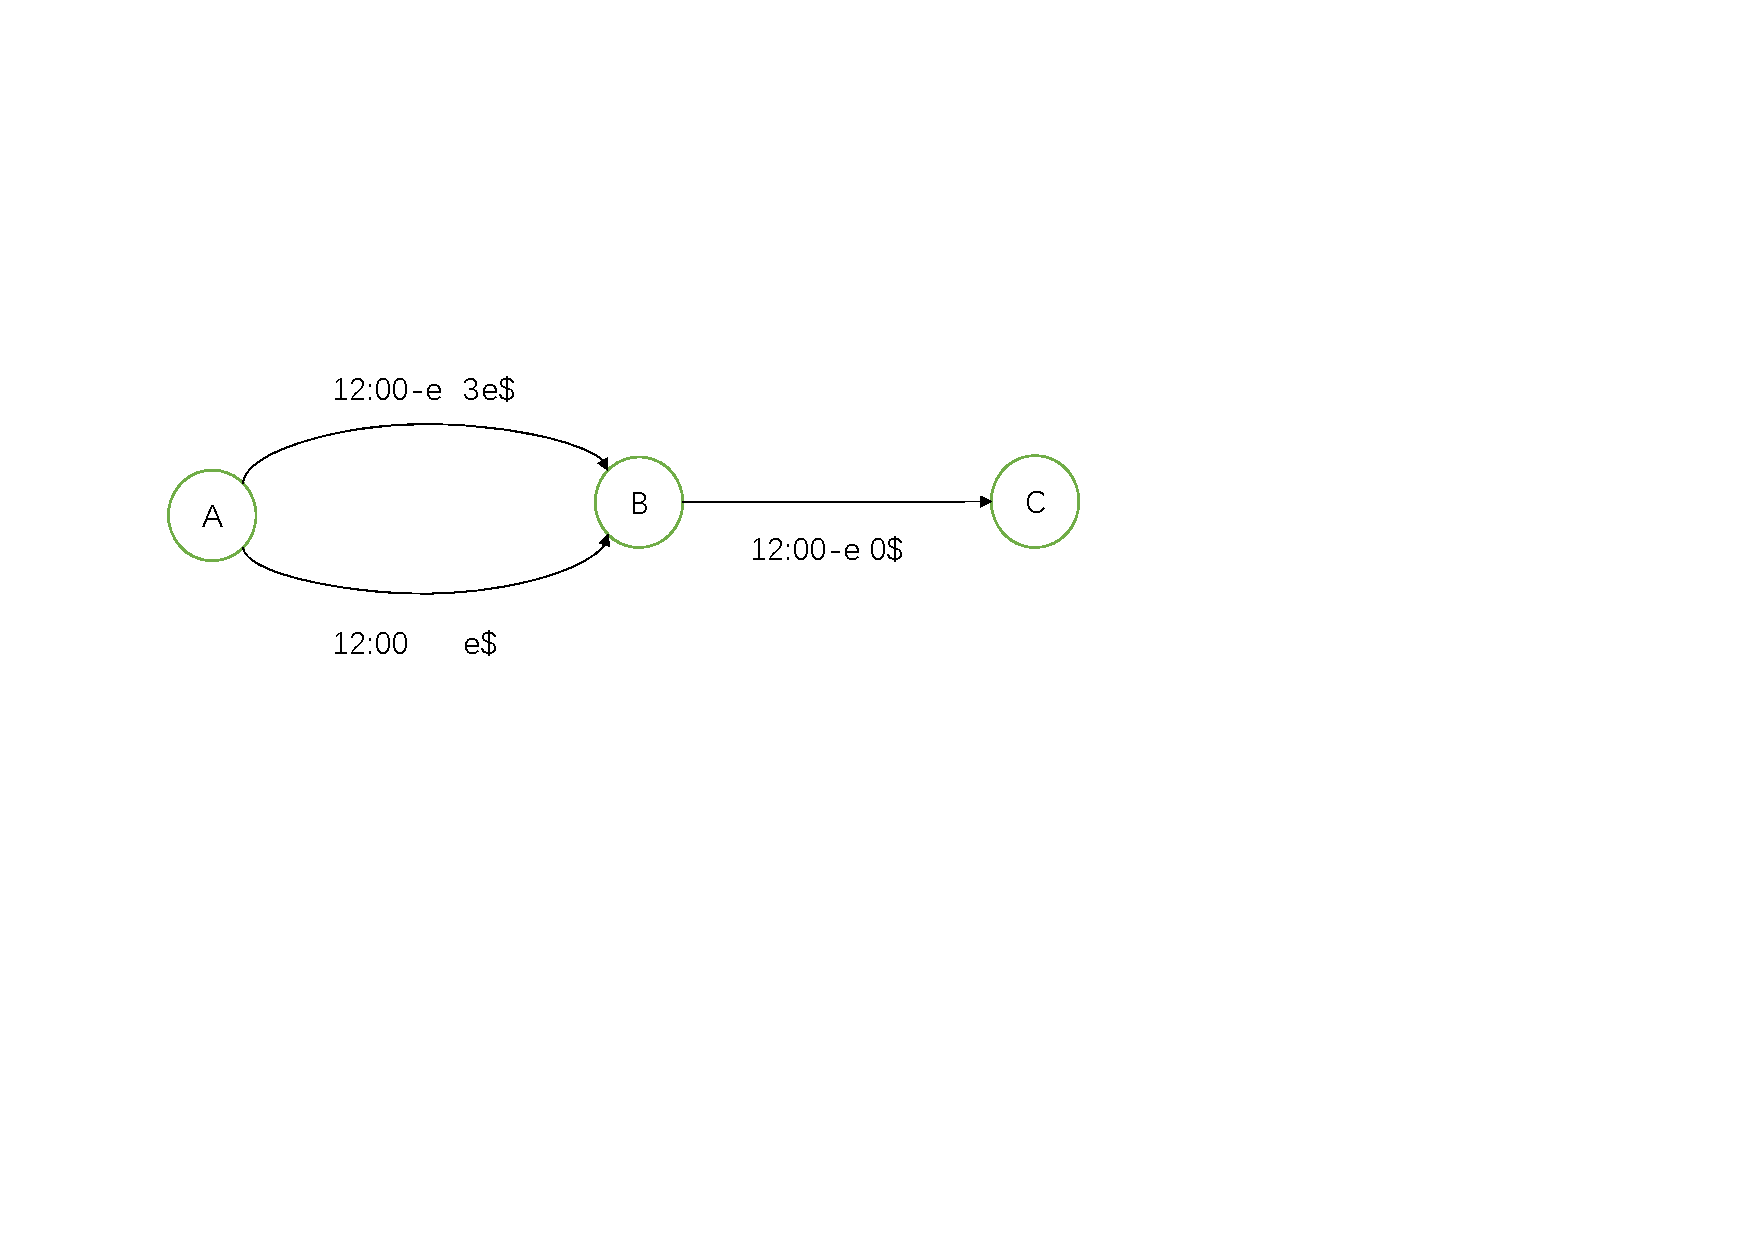
\includegraphics[width=\textwidth]{figure/citynetwork1}
			\caption{city network 1}
			\label{fig:ct1}
		\end{figure}
		\item Approximation Difference\par
		$\quad$ Then we use another criterion approximation difference to evaluate the lower bound of the performance. Approximation difference is defined as $\max\{f(dijskra)-f(OPT)\}$. This criterion is more appropriate for this problem than approximation ratio. This is because users care about how much time the package is late for. And the company cares about how much money they waste. They care the difference rather than the ratio. 
		
		$\quad$ Using this criterion, the algorithm is $poly-apx$. I.e. $\max\{f(dijskra)-f(OPT)\}$ is a polynomial function of the input. Denote the number of cities as $k$. The approximation difference is $1440b(k-1)$. Notice that the number of minutes in a day is 1440. Proof: if we don't care the waiting time, $dijskra$ is no worse than $OPT$. And the maximum time $dijskra$ waste on waiting is when it go through all $k$ cities in a delivery and wait for about a day on each edge. Then the time wasted is $1440(k-1)$. This causes $1440b(k-1)$ difference to $f$.
		
		$\quad$ This lower bound seems to be exaggerated. But it's actually a tight bound. See the network in figure \ref{fig:ct2}. $time\_on\_way=0$ for all edges and the order happens at $12:00-3$. $OPT$ chooses the above edges for all, while $dijskra$ chooses the below ones. Then the $dijskra$ reaches $k$ $k-1$ days later, while $OPT$ reaches $k$ immediately. If we choose $e$ arbitrarily little, the approximation difference can be arbitrarily close to $1440(k-1)$.
		\begin{figure}
			\centering
			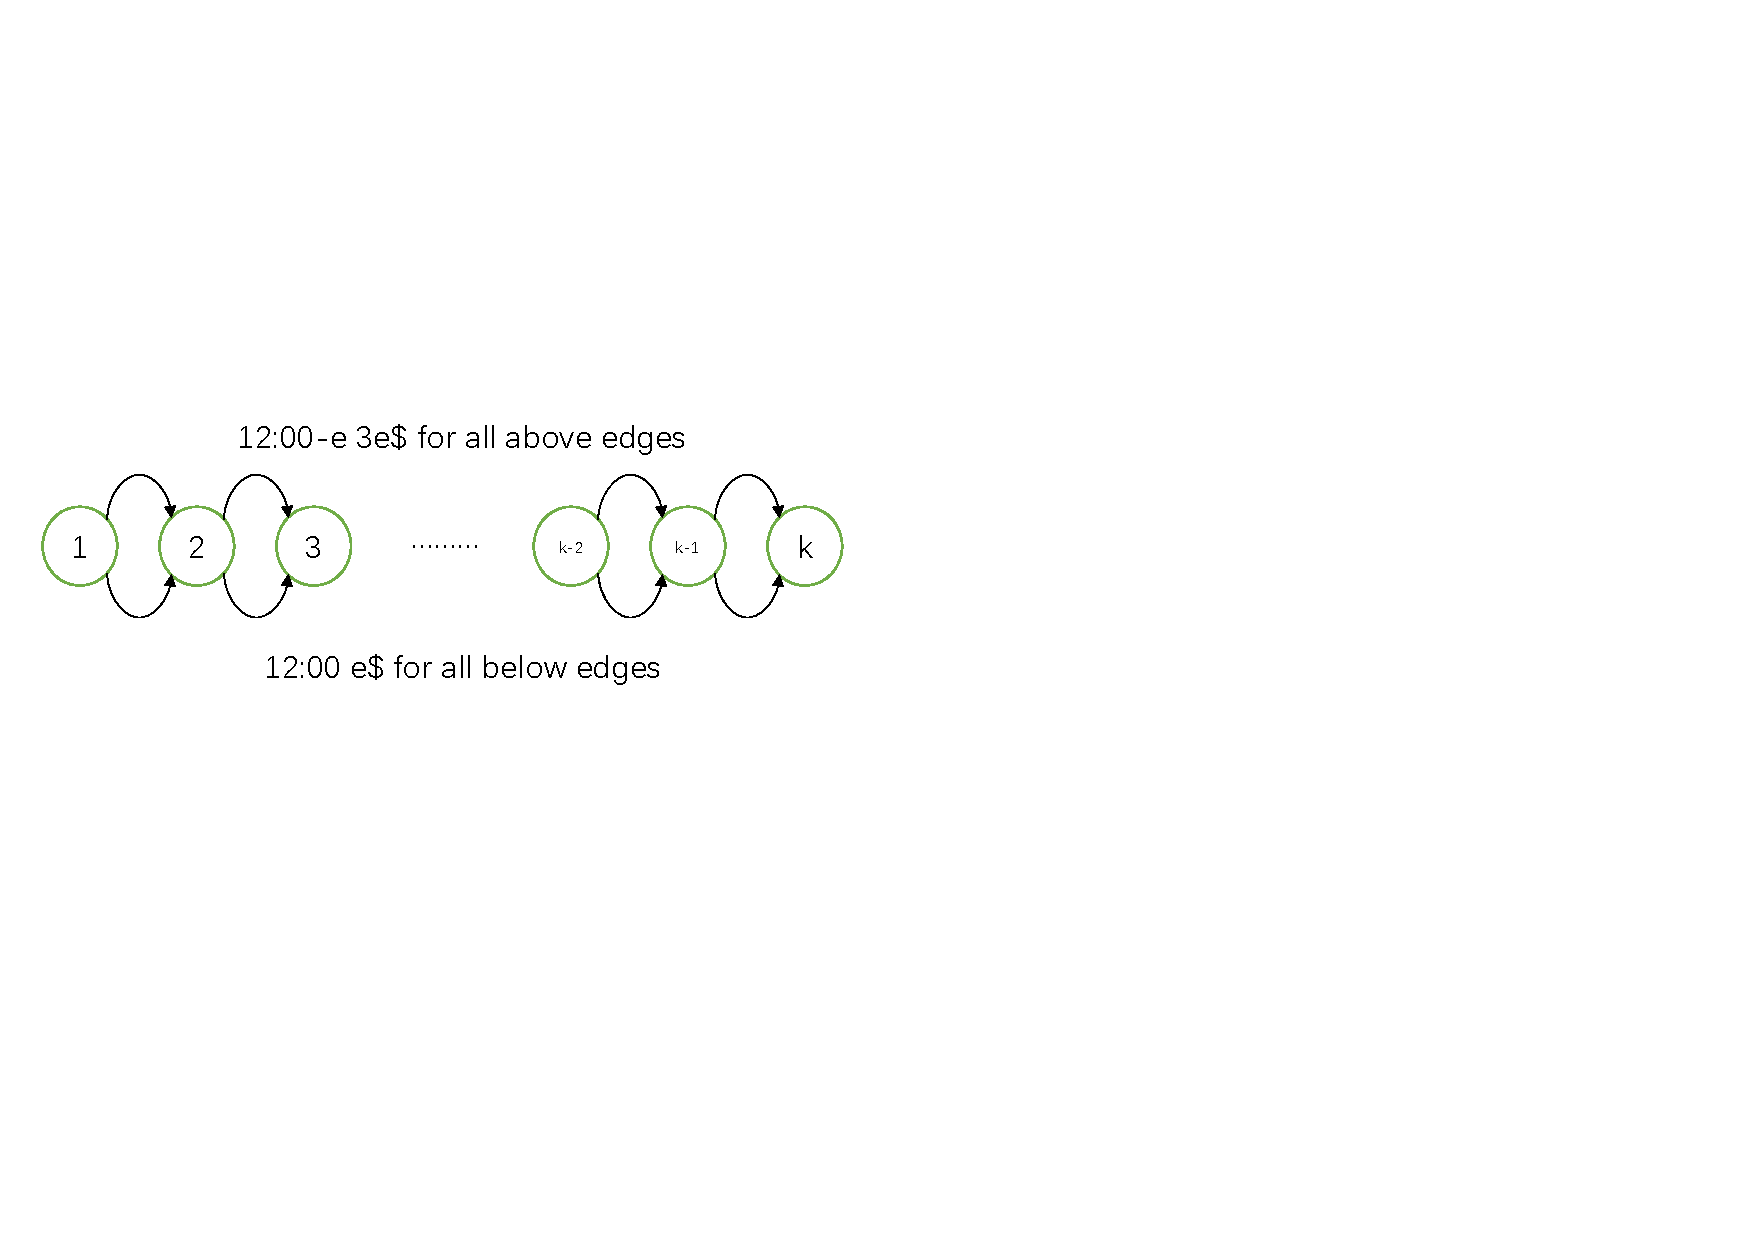
\includegraphics[width=\textwidth]{figure/citynetwork2}
			\caption{city network 2}
			\label{fig:ct2}
		\end{figure}
		\item Analysis in practice
		The $poly-apx$ seems to be terrible, but actually this algorithm works well in practice. This is because the real-world city network is a dense graph rather than the 1-dimension one shown in figure \ref{fig:ct2}. And the probability that $dijskra$ chooses such a long path is nearly 0.
		
		$\quad$ In fact, we run the algorithm on the given city network. The largest $f$ we get is $$158885.46 = 18\times 8676.70 + 1.2\times 2254.05.$$ We choose $a=18$ and $b=1.2$ in practice. This order costs 8760.70\$ and uses about one day and a half. This is far lower than using $k-1$ days. Therefore, the algorithm works well in practice.

	\end{enumerate}
	
	\subsection{Efficiency Analysis}
	For each order, we run $dijskra$ once. Use $array$ for implementation. The algorithm checks each transportation tool at most once. Each check is $O(1)$. Also, each $edge$ and $vertex$ in $G$ is checked at most once. Denote the total number of transportation tools in TableD-TransportationTools by $\#tools$. Denote the vertices set and edges set in $G$ by $V$ and $E$. Then the time complexity is $O(\#tools+|V|+|E|)$. Also, find the city with the lowest $OPT\_value$ is $O(|V|)$ in array implementation. Therefore, the time complexity is $O(\#tools+|V|^2)$. For each order, the algorithm runs once. Hence, the total time complexity is $O((\#tools+|V|^2)\times |orders|)$.
\section{Problem 2}
	\subsection{Problem Analysis}\label{2-PA}
	Assume the cost to construct a hub is $\hat{c}$. 
	$$\hat{c}=c_0+c_1|orders|$$
	$c_0$ is the cost for building the hub (a constant). $c_1|orders|$ is the cost for running the hub. $|orders|$ is the number of orders going through the hub. This is proportional with  $|orders|$.
	
	And assume the transportation cost between two hubs is $x(0\leq x\leq 1)$ times that not between hubs. The $f$ of a delivery is the sum of all the $f$s of its route.\par
	\indent For simplicity, \textbf{we assume that the delivery routes remain unchanged and only consider how to set up hubs and which transportation tool to use.} The idea is to sequentially check whether setting up a hub in a city can optimize $f(time,cost)$.
	
	\subsection{Problem Formulation and Complexity Analysis}
	We formulate this problem by $(I,sol,m,goal)$.
	\begin{itemize}
		\item $I$ : $(G,orders,paths,\hat{c},x)$. $G$ is a city network. $orders$ is the set of orders. $paths$ is the scheme generated in problem 1. $paths$ is denoted by $|orders|$ paths in graph $G$. $x$ and $\hat{c}$'s meaning are shown in section \ref{2-PA}. This is poly-time recognizable.
		\item $sol$ : $sol(G,orders,paths,\hat{c},x)$ is the set of $(m\_paths,hubs)$. The requirements are:(i) the routes in $m\_paths$ is the same with that in $paths$ (transportation tools can be different); (ii) from one $hub\in hubs$ to one city, there is only one transportation tool used. This is also poly-time recognizable.
		\item $m$ : The overall evaluation of scheme $paths$ is denoted by $sum\_f(paths)$. The overall evaluation of scheme $m\_paths$ is denoted by $sum\_f(m\_paths)$. Then $m(m\_paths, hubs) = sum\_f(paths)-sum\_f(m\_paths)$. I.e. the reduced amount of $sum\_f$. This is poly-time calculatable.
		\item $goal$ : maximize.
	\end{itemize}
	Therefore, we've shown that this is a NP-problem.
	\subsection{Algorithm Design}
	Since the orders and their routes have been solved in Problem $1$, we have already known how many things of each type go through each city. We have also been restricted to using only one transportation tool from the hub to one city. So the transportation from the hub through different transportation tools has to be merged. Another check of which means of transportation is the best choice is therefore required. Algorithm \ref{alg:ck2} is the one checking whether construct a hub in city $C$. Algorithm \ref{alg:st-noapp} and \ref{alg:st} are 2 versions of the outer algorithms.
	
	\begin{algorithm}\label{alg:ck2}
		\caption{check($C$, $H$, $paths$)}
		\KwIn{City $C$, current hub set $H$, current scheme $paths$;}
		\KwOut{The benefit from building a hub in city $C$, new scheme $paths$;}
		\BlankLine
		//Notice that when calculating $sum\_f$, simulate the whole process, and take $H$ into consideration\;
		$benefit\leftarrow 0$\;
		\ForEach{City $C'$ reachable from $C$}
		{
			$max\_benefit\leftarrow 0$\;
			\ForEach{$tool\in tools$ from $C$ to $C'$}
			{
				$m\_paths$ $\leftarrow$ $paths$ but make all commodities from $C$ to $C'$ transported by $tool$\;
				\If{$sum\_f(paths)-sum\_f(m\_paths)$>$max\_benefit$}
				{
					
					$max\_benefit\leftarrow sum\_f(paths)-sum\_f(m\_paths)$\;
					$opt\_paths\leftarrow m\_paths$\;
				}
			}
			$paths\leftarrow opt\_paths$\;
			$benefit+=max\_benefit$\;
		}
		\Return{($benefit-\hat{c}$,$paths$)}\;
	\end{algorithm}
	
	\begin{algorithm}\label{alg:st-noapp}
		\caption{$Set\_up\_hubs1(S,paths)$}
		\KwIn{$S$ a set of cities, scheme $paths$ got in problem 1}
		\KwOut{$H$ a set of hubs, new scheme $paths$;}
		\BlankLine
		$H\leftarrow\emptyset$\;
		\For{$c\in S$}
		{
			\If{$check(c,H,paths).benefit>0$}{
				$H\leftarrow H\cup\{c\}$\;
				$paths\leftarrow check(c,H,paths).paths$\;
			}
		}
		\Return{($H$,$paths$)}\;
	\end{algorithm}
	
	\begin{algorithm}\label{alg:st}
		\caption{$Set\_up\_hubs2(S,paths)$}
		\KwIn{$S$ a set of cities,scheme $paths$ in problem 1;}
		\KwOut{$H$ a set of hubs, new scheme $paths$;}
		\BlankLine
		$H\leftarrow\emptyset$\;
		\While{$H\neq S$}
		{
			$max\_benefit\leftarrow 0$\;
			\For{$c\in S/H$}
			{
				\If{$check(c, paths).benefit>max\_benefit$}
				{
					$max\_benefit\leftarrow check(c, paths).benefit$\;
					$max\_city\leftarrow c$\;
				}
			}
			\If{$max\_benefit\leq 0$}
			{
				break\;
			}
			\Else
			{
				$H\leftarrow H\cup \{max\_city\}$\;
				$paths\leftarrow$ the scheme by setting $max\_city$ as a hub\;
			}
		}
	
		\Return{($H$,$paths$)};
	\end{algorithm}
	\subsection{Performance Analysis}
	Notice that neither algorithm \ref{alg:ck2} nor \ref{alg:st} guarantees optimal solution. They are both sequential algorithms. Algorithm \ref{alg:ck2} sequentially determine the transportation tool from $C$ to each city. Algorithm \ref{alg:st} sequentially determine whether constructing a hub in each city. However, the determination in previous iteration changes the scheme $paths$, thus influencing the later determinations. I.e. the order in which the cities are checked actually influence the outcome. Hence, the optimal solution is not guaranteed.
	
	We gave 2 versions of the outer algorithm. Algorithm \ref{alg:st-noapp} simply checks each city and determine whether to make it a hub. This may lead to an arbitrarily bad result. E.g. it chooses the first city with very little benefit. However this choice makes all other cities unable to be hubs ($benefit\leq 0$). But the $OPT$ can achieve much more benefit. To make this situation impossible, we also design another algorithm \ref{alg:st}.
	
	Algorithm \ref{alg:st} is poly-apx ($k-apx$). $k$ is the number of cities. The benefit achieved by algorithm \ref{alg:st} is at least the benefit of constructing the first $max\_city$. I.e. $max\_benefit$ in the first iteration. The benefit achieved by $OPT$ is at most $k\times max\_benefit$. I.e. constructing hubs in each city and each with benefit the same as $max\_benefit$. Therefore, we get the following formula:
	$$
	\frac{OPT.benefit}{sequential.benefit}<\frac{k\times max\_benefit}{max\_benefit}=k.
	$$
	Hence, algorithm \ref{alg:st} is poly-apx.
	
	\subsection{Efficiency Analysis}\label{sec:2-E}
	The function $check$ is $O(\#tools_C\times |E|\times |orders|)$. $\#tools_C$ is the number of transportation tools from city $C$. $|E|$ is the number of edges in graph $G$. This is because that the algorithm simulates to get benefit $\#tools_C$ times. And each simulation requires $O(|E|\times |orders|)$ time.
	
	For algorithm \ref{alg:st-noapp}, the time complexity is $O(\#tools\times |E|\times |orders|)$. $\#tools$ is the total number of transportation tools. This is because adding up $\#tools_C$ for each city reaches $\#tools$. 
	
	For algorithm \ref{alg:st}, the time complexity is $O(\#tools\times |E|\times |orders| \times |V|)$. $|V|$ is the number of vertices in $G$. This is because we check each city for at most $|V|$ times.
	
	Since algorithm \ref{alg:st} is much slower, we implemented algorithm \ref{alg:st-noapp} instead.
	
	We can improve the efficiency by only checking the orders whose delivery scheme has changed. However, this won't change the complexity in the worst case. This is because in the worst case, all orders go through all cities. Hence, when the transportation tools are merged, all orders' delivery schemes changed. Anyway, this optimization works well in practice.

\section{Problem 3}
\subsection{Problem Analysis}
	For this problem we assume that the hub and the substation can function in the same city since hubs are capacitied. This is quite similar to problem $2$ except that a little change has to be made to the algorithm to check for each city. Obviously, this is still a NP problem.
\subsection{Algorithm Design}
	Since the hubs are capacitied, we have to take this into consideration and decide which commodities are to be transported 
	through hubs and which through substations. 
	
	First, we should determine which orders to be delivered by the hub in the city. To maximize the benefit from the hub, we can treat the time and money we save as the value and the order's commodity's weight as the weight. Then convert the problem into a knapsack problem. The algorithm \ref{alg:knap} illustrates our idea.
	
	\begin{algorithm}\label{alg:knap}
		\caption{$checkTool(C,C',T)$}
		\KwIn{Cities $C$ and $C'$ in which $C'$ is reachable from $C$ by $T$, a transportation tool;}
		\KwOut{The maximum benefit of delivery from $C$ to $C'$ if we build a hub in city $C$ and use $T$ to deliver the goods;}
		\BlankLine
		\For{Commodity $c$ going through $C$ that are allowed in the hub of $C$ and in $T$}
		{
			$value[c]=f(p')-f(p)$ in which $p$ is the path with the old transportation while $p'$ goes by the new one\;
			$r[c]=\dfrac{value[c]}{weight[c]}$\;
		}
		$b\leftarrow$ The capacity of the hub\;
		Sort $r$ in non-increasing order $r_1,r_2,\ldots,r_k$\;
		$benefit\leftarrow0$\;
		\For{$i\leftarrow 1$ to $n$}
		{
			\If{$b\geq weight[c_i]$}
			{
				$c\leftarrow\max_c\{value_{max},r_i\}$\;
			}
			\Else
			{
				$c\leftarrow\max_c\{value\}$\;
				\If{$b<weight[c_i]$}
				{
					$c\leftarrow null$\;
				}
			}
			Put $c$ into the hub\;
			$benefit\leftarrow benefit+value[c]$\;
			$b\leftarrow b-weight[c]$\;
		}
		\If{$benefit$ < the benefit of putting only the feasible order with the largest $value$}
		{
			Only put the feasible order with the largest $value$ instead\;
		}
		\Return{$benefit$};
	\end{algorithm}
	Then we can give the modified algorithm $check$ in algorithm \ref{alg:ck}
	\begin{algorithm}\label{alg:ck}
		\caption{check($C$)}
		\KwIn{City $C$;}
		\KwOut{The overall benefits from building a hub in city $C$;}
		\BlankLine
		$benefit\leftarrow-\hat{c}$\;
		\For{City $C'$ reachable from $C$}
		{
			$c\leftarrow\min_{T\in\text{Available tools from }C\text{ to }C'}checkTool(C,C',T)$\;
			$benefit\leftarrow benefit+(\text{the current total f(time,cost) from}C\text{ to }C')-c$\;
		}
		\Return{$benefit$};
	\end{algorithm}

	And the outer algorithm remains unchanged.
	
	Notice that when calculating the benefit, let those glass-made or inflammable products transported via the substation rather than hub in those cities which don't allow them.  Also, the original scheme needs to be changed. For those orders with liquid and inflammable products, run the algorithm in problem 1 again, adding the constraint. Then run algorithms on the modified original scheme. Anyway, these 2 constraints will not cause substantial difference to our model.
	\subsection{Performance Analysis}
	The approximation ratio changes to $2k$, which is still poly-apx. This ratio is got by multiplying the ratio in problem 2 by 2. In class, we are taught that the knapsack problem is with approximation ratio 2. Hence multiply the approximation ratio in the 2 procedure and we got the overall approximation ratio.
	
	\subsection{Efficiency Analysis}
	 Use the symbols defined in section \ref{sec:2-E}. The time complexity of algorithm \ref{alg:knap} is $O((|E|+\log{|orders|})|orders|)$. Calculating each order's value is $O(|E||orders|)$. Sorting the orders is $O(|orders|\log{|orders|})$.
	
	The complexity changes because each check takes more time. The check function's complexity becomes $O(\#tools_C(|E|+\log{|orders|})|orders|)$.
	
	Then the complete algorithm's time complexity is $O(\#tools(|E|+\log{|orders|})|orders|)$ (algorithm \ref{alg:st-noapp}) or $O(\#tools(|E|+\log{|orders|})|orders||V|)$ (algorithm \ref{alg:st}).

\section{Problem 4}

	\subsection{Problem Analysis}
	Here is our assumption for this problem. If the $seller\_city$ is not a substation, it should be first delivered to a $substation$. As soon as the commodity reaches any substation, it should be delivered between substations, i.e. not going back to small cities. Once the commodity goes back to some small city, it should be transported to $purchaser\_city$ without going back to any substations. I.e. the commodities should be transported first between small cities, then substations and then again small cities. This is close to the reality.\par
	Moreover, in reality those substations should be reachable from each other without small cities as intermediate. Otherwise, some substations may become islets. And any small city should be reachable from and to at least one substation. Otherwise, the city becomes an islet. Therefore, we make these 2 as our requirements for the data set.\par
	\indent We can revise our model by only set those cities with substations as the vertices. For those small cities without substations, associate them with the nearest substation. I.e. construct ``huge vertices''.
	
	\subsection{Complexity Analysis}
	Actually $problem_4\leq _pproblem_1$. Since for the situation where $seller\_city$ and $purchaser\_city$ are neither substation. All feasible delivery delivers from $seller\_city$ to substation $s$ and then to substation $t$ and finally to $purchaser\_city$. ($s$ can be the same substation as $t$). Then we can let the algorithm exhaust all the possibilities of the choices of $s$ and $t$. There are at most $O(|cities|^2)$ possibilities. Therefore, running the algorithms this many time can solve problem 4.
	
	\subsection{Modeling}
	\begin{itemize}
		\item Modeling cities\par
		$\quad$ A city is modeled by a pair $$(index, attribute).$$ $index$ is the city's index. $attribute$ can be $substation$ or $small$.
		
		\item Modeling graph\par
		$\quad$ In this problem, we construct 2 graphs $G$ and $G_r$. $G$ is the same graph with problem 1. For $G_r$, delete all the cities without substation from the $G$ in problem 1. And delete corresponding edges.
	\end{itemize}
	
	
	\subsection{Algorithm Design}
	Although exhausting all probabilities can reach an optimized solution, it's too inefficient. Therefore, we revise the algorithm to be algorithm \ref{alg:4}. Notice that theoretically this may lead to arbitrarily bad result. E.g. $seller\_city$ is not a substation but $purchaser\_city$ is. However the nearest substation from $seller\_city$ is infinitely far from the $purchaser\_city$. However, this can never happen in reality since the triangle law on real-world map. Therefore, this algorithm can lead to very close answer to the OPT in practice.\\
	\begin{algorithm}[H]\label{alg:4}
		\caption{Schedule($G$,$order$)}
		\KwIn{city network $G$ and an order $order$.}
		\KwOut{A path from $order.seller\_city$ to $order.purchaser\_city$}
		\BlankLine
		\ForEach{$(u,v)\in E(G)$}
		{
			Weight the edge by $Weight(u,v,G,order).minweight$\;
		}
		\ForEach{$(u,v)\in E(G_r)$}
		{
			Weight the edge by $Weight(u,v,G_r,order).minweight$\;
		}
		$G_{rr}\leftarrow$ graph $G$ deleting all substations\;
		$substation\_s\leftarrow order.seller\_city$\;
		$substation\_t\leftarrow order.purchaser\_city$\;
		\If{$order.seller\_city.attribute==substation$ \&\& $order.purchaser\_city.attribute==subtation$}
		{
			Run Algorithm \ref{alg:search} in problem 1 on $G_r$\;
			\Return{the path got}\;
		}
		\If{$order.seller\_city.attribute==small$}
		{
			Use $dijskra$ on $G_{rr}$ to calculate the shortest path from $order.seller\_city$ to each small city\;
			\ForEach{small city}
			{
				Update the shortest distance of neighbor substations\;
			}
			Choose the substation $s_m$ with minimum weight of the shortest path\;
			$substation\_s\leftarrow s_m$\;
		}
		\If{$order.purchaser\_city.attribute==small$}
		{
			Use $dijskra$ on $G_{rr}$ to calculate the shortest path from  each small city to $order.purchaser\_city$ \;
			\ForEach{small city}
			{
				Update the shortest distance of neighbor substations\;
			}
			Choose the substation $t_m$ with minimum weight of the shortest path\;
			$substation\_t\leftarrow t_m$\;
		}
		Run $dijskra$ algorithm $G_r$ to find a shortest path from $substation\_s$ to $substation\_t$\;
		Combine the 3 paths as $path$\;	
		\Return{$path$}\;
	\end{algorithm}
	The algorithm's complexity is also
	$$
	T(|orders|,\#cities)=|orders|\times \#cities^2.
	$$
%----------------------------------------------------------------------------------------
% Research design
%----------------------------------------------------------------------------------------

\section{Performance Evaluation}
\subsection{Delivery Scheme}
	The entire result is available on http://resources.dbgns.com/package-delivery/results.
\begin{enumerate}
	\item Problem 1\\
	We run the algorithm for every order and got their delivery schemes. We list some as follow. 
	\begin{verbatim}
	For order 0 with totalWeight: 187.529 and emergency: 0, Best strategy is:
	Paths: [655, 614, 593, 10], Vehicles: ['Truck', 'Truck', 'Truck'], 
	AmountCost: 200.161$, TimeCost: 584.11m, ArrivalTime: 23:50:55
	
	For order 33 with totalWeight: 7.612 and emergency: 0, Best strategy is:
	Paths: [362, 621, 73, 646], Vehicles: ['Plane', 'Truck', 'Truck'], 
	AmountCost: 18.661$, TimeCost: 685.48m, ArrivalTime: 23:33:39
	\end{verbatim}
	\item Problem 2\\
	In this problem, the delivery scheme will change because of the constraints of hubs. And we only list the cities where we construct hubs here. 4 hubs are constructed in total.
	\begin{verbatim}
	106 205 164 503 
	\end{verbatim}
	\item Problem 3\\
	Also, we list the cities where we construct hubs here. 32 hubs are constructed in total.
	\begin{verbatim}
	358 400 290 406 549 417 529 577 187 106 51 308 651 531 183 252
	205 469 223 164 503 117 199 197 370 352 524 449 460 424 397 302 
	\end{verbatim}
	\item Problem 4\\
	Since the constraints added, the delivery schemes change. E.g. order 0's scheme changed to:
	\begin{verbatim}
	For order 0 with totalWeight: 187.529 and emergency: 0, Best strategy is:
	Paths: [10, 548, 170, 54, 655, 403, 170],
	Vehicles: ['Truck', 'Truck', 'Ship', 'Truck', 'Truck', 'Truck'], 
	AmountCost: 343.953$, TimeCost: 5398.69m, ArrivalTime: (+4day):8:05:30
	\end{verbatim}
\end{enumerate}
\subsection{Ratio of Transportation Tools}
	In this section, we visualized the ratio of transportation tools for each problem. See figure \ref{fig:p1}, \ref{fig:p2}, \ref{fig:p3} and \ref{fig:p4}. From this figure, we found that truck occupied a huge ratio of chosen transportation tools. And plane occupies very little. One reason is that the number of trucks is far more than that of other transportation tools. Another reason is that plane is too expensive. And this also correspond with reality. Since in reality, only emergency packages will be transported by plane. Another interesting result is that, in problem 4, ship occupied a substantially larger ratio.
	\begin{figure}
		\centering
		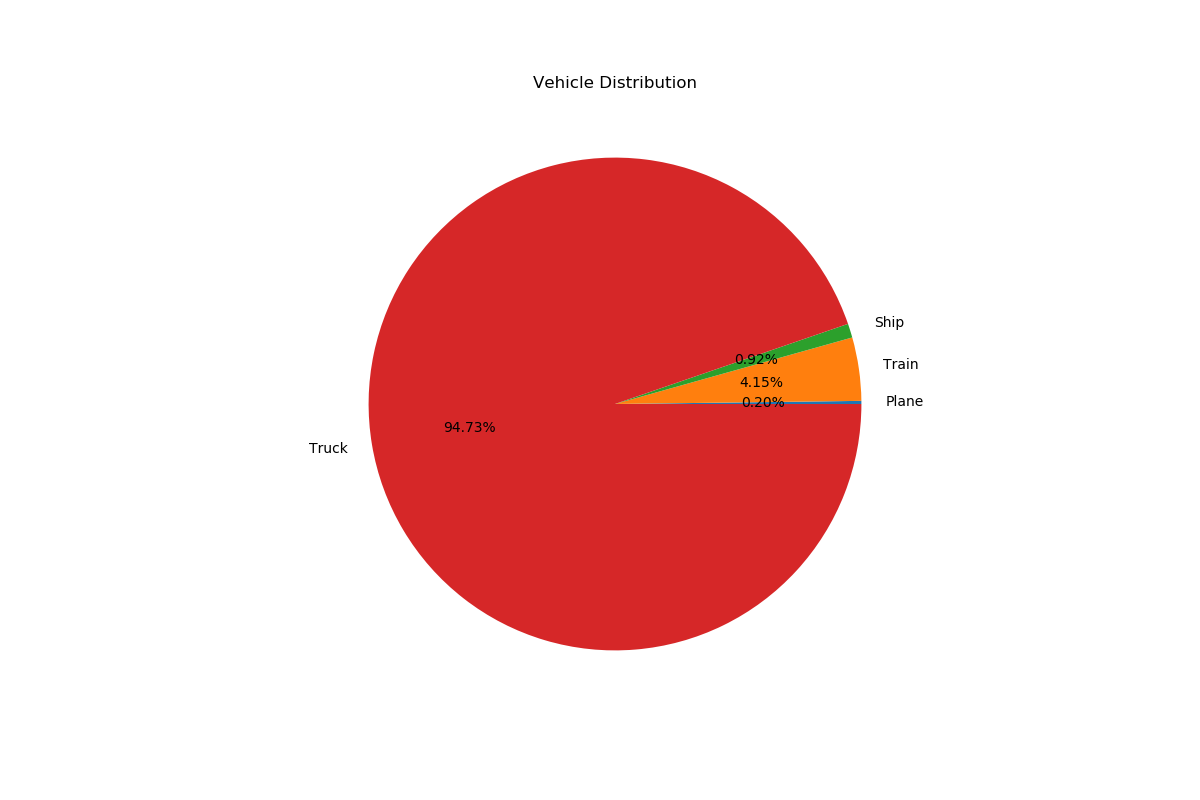
\includegraphics[width=0.8\linewidth]{figure/vehicle1.png}
		\caption{problem 1}
		\label{fig:p1}
	\end{figure}
	\begin{figure}
		\centering
		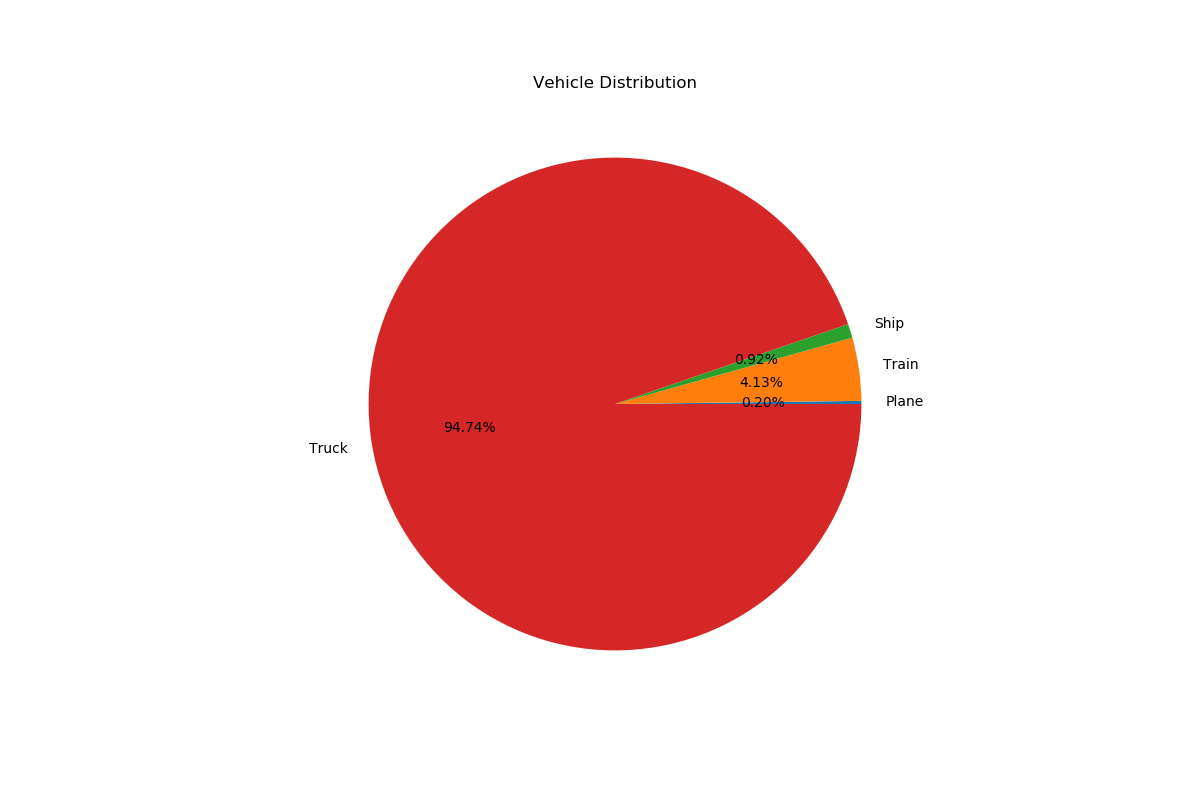
\includegraphics[width=0.8\linewidth]{figure/vehicle2.png}
		\caption{problem 2}
		\label{fig:p2}
	\end{figure}
	\begin{figure}
		\centering
		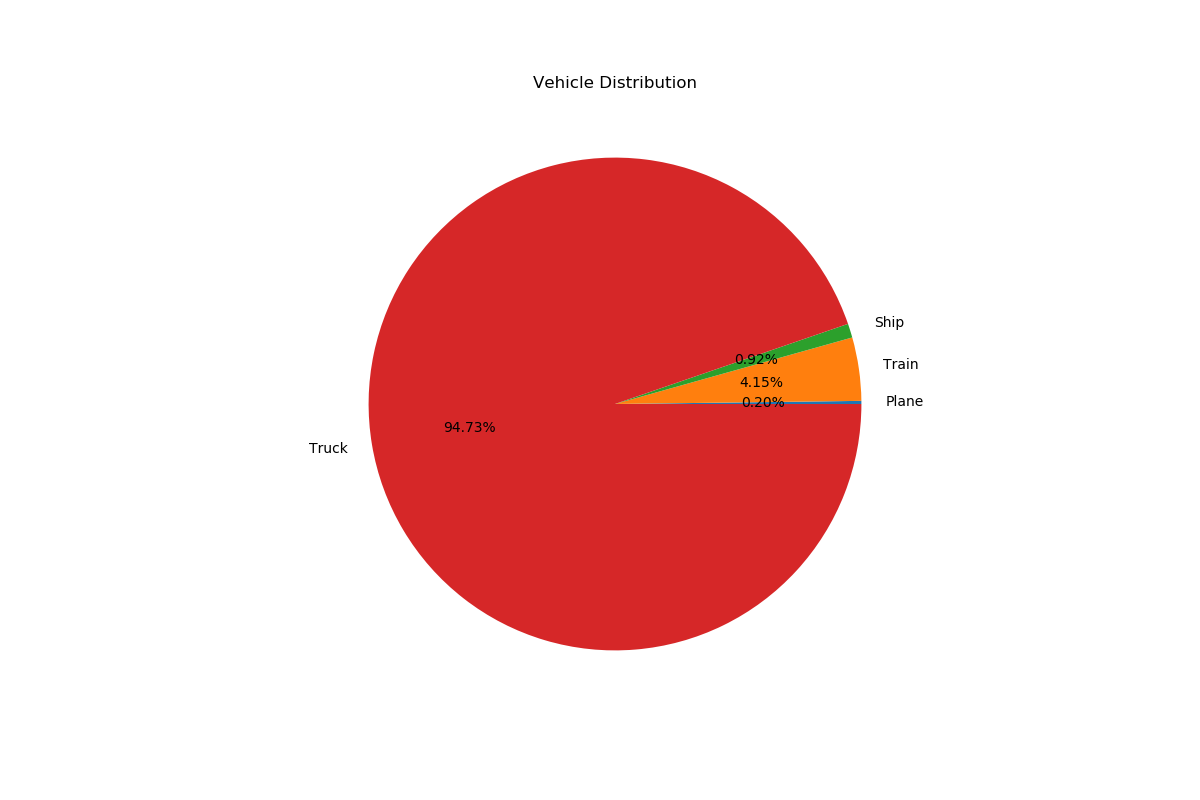
\includegraphics[width=0.8\linewidth]{figure/vehicle3.png}
		\caption{problem 3}
		\label{fig:p3}
	\end{figure}
	\begin{figure}
		\centering
		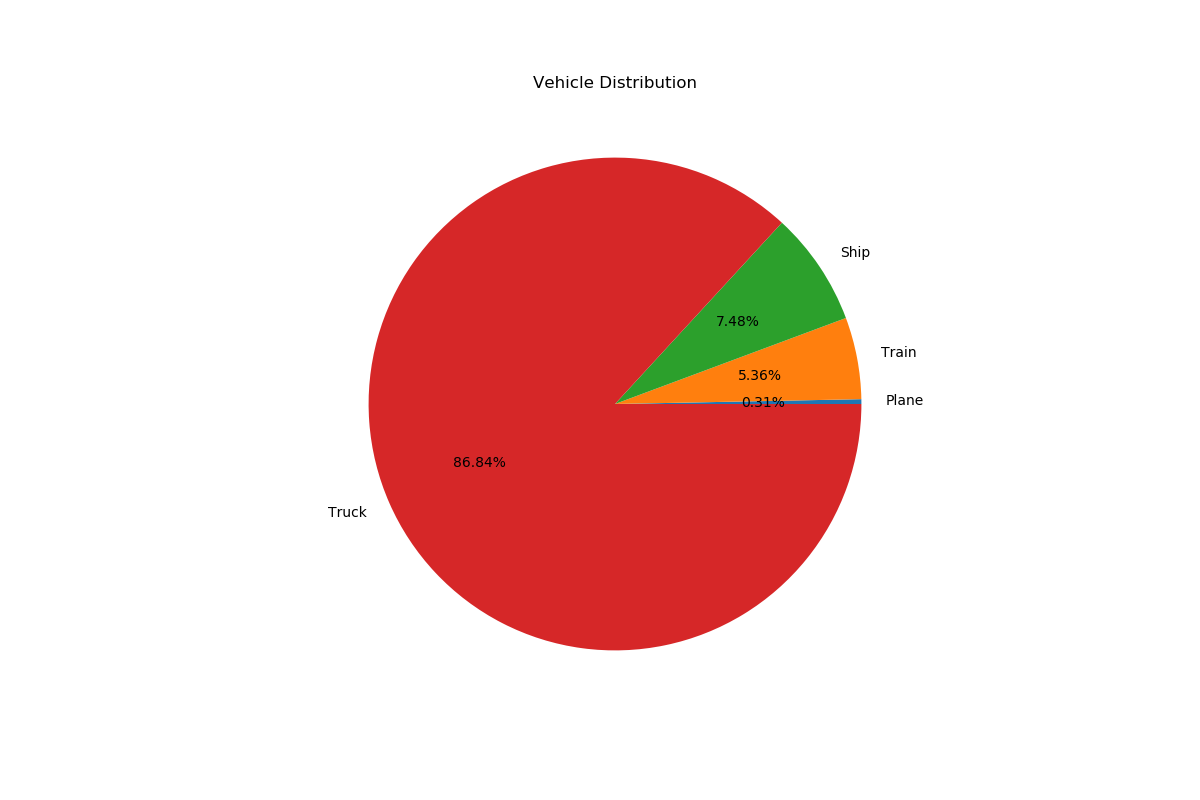
\includegraphics[width=0.8\linewidth]{figure/vehicle4.png}
		\caption{problem 4}
		\label{fig:p4}
	\end{figure}

\subsection{Trade-off Between Customer Rating and Cost}
	We changed parameters $a$ and $b$. ($f=a\times cost+b\times time$.) Under different parameters, use $a/b$ as independent variable. And use $cost$ and $time$ as dependent variables. We get the figure \ref{fig:tradeoff}. 
	
	$AmountCost$ corresponds to $cost$ and $timeCost$ corresponds to $time$. From this figure, we found that as $a/b$ increases, $time$ and $cost$ increases and decreases respectively. Therefore, there is actually a trade-off between customer rating and cost.
	\begin{figure}
		\centering
		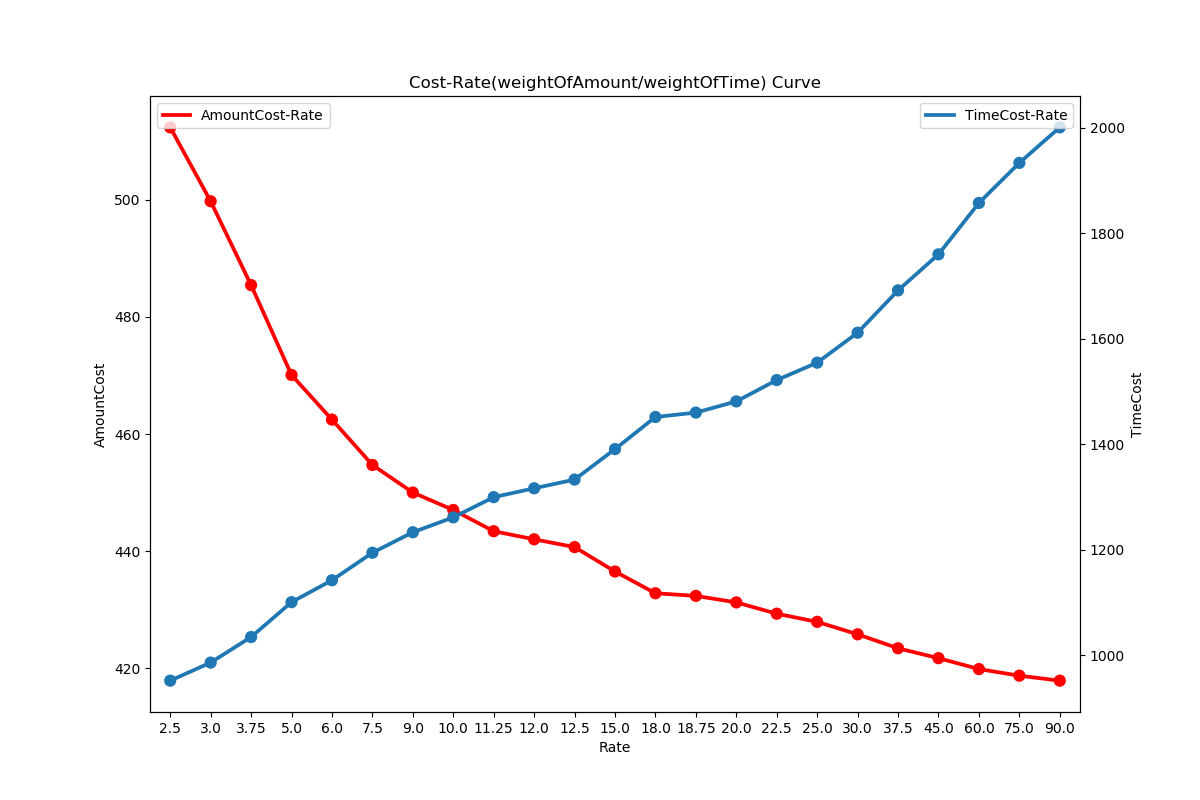
\includegraphics[width=\linewidth]{figure/tradeoff.png}
		\caption{Trade of between customer rate and cost}
		\label{fig:tradeoff}
	\end{figure}

	Since there is a trade-off between them, maybe we need to determine $a$ and $b$ more carefully to strike a balance between them. The objective is to achieve lower $time$ and $cost$. Hence, we use $time\times cost$ achieved by the algorithm as the dependent variable. And use $a$ and $b$ as independent variables. Then the relationship between them is shown in figure \ref{fig:ab}
	\begin{figure}
		\centering
		
		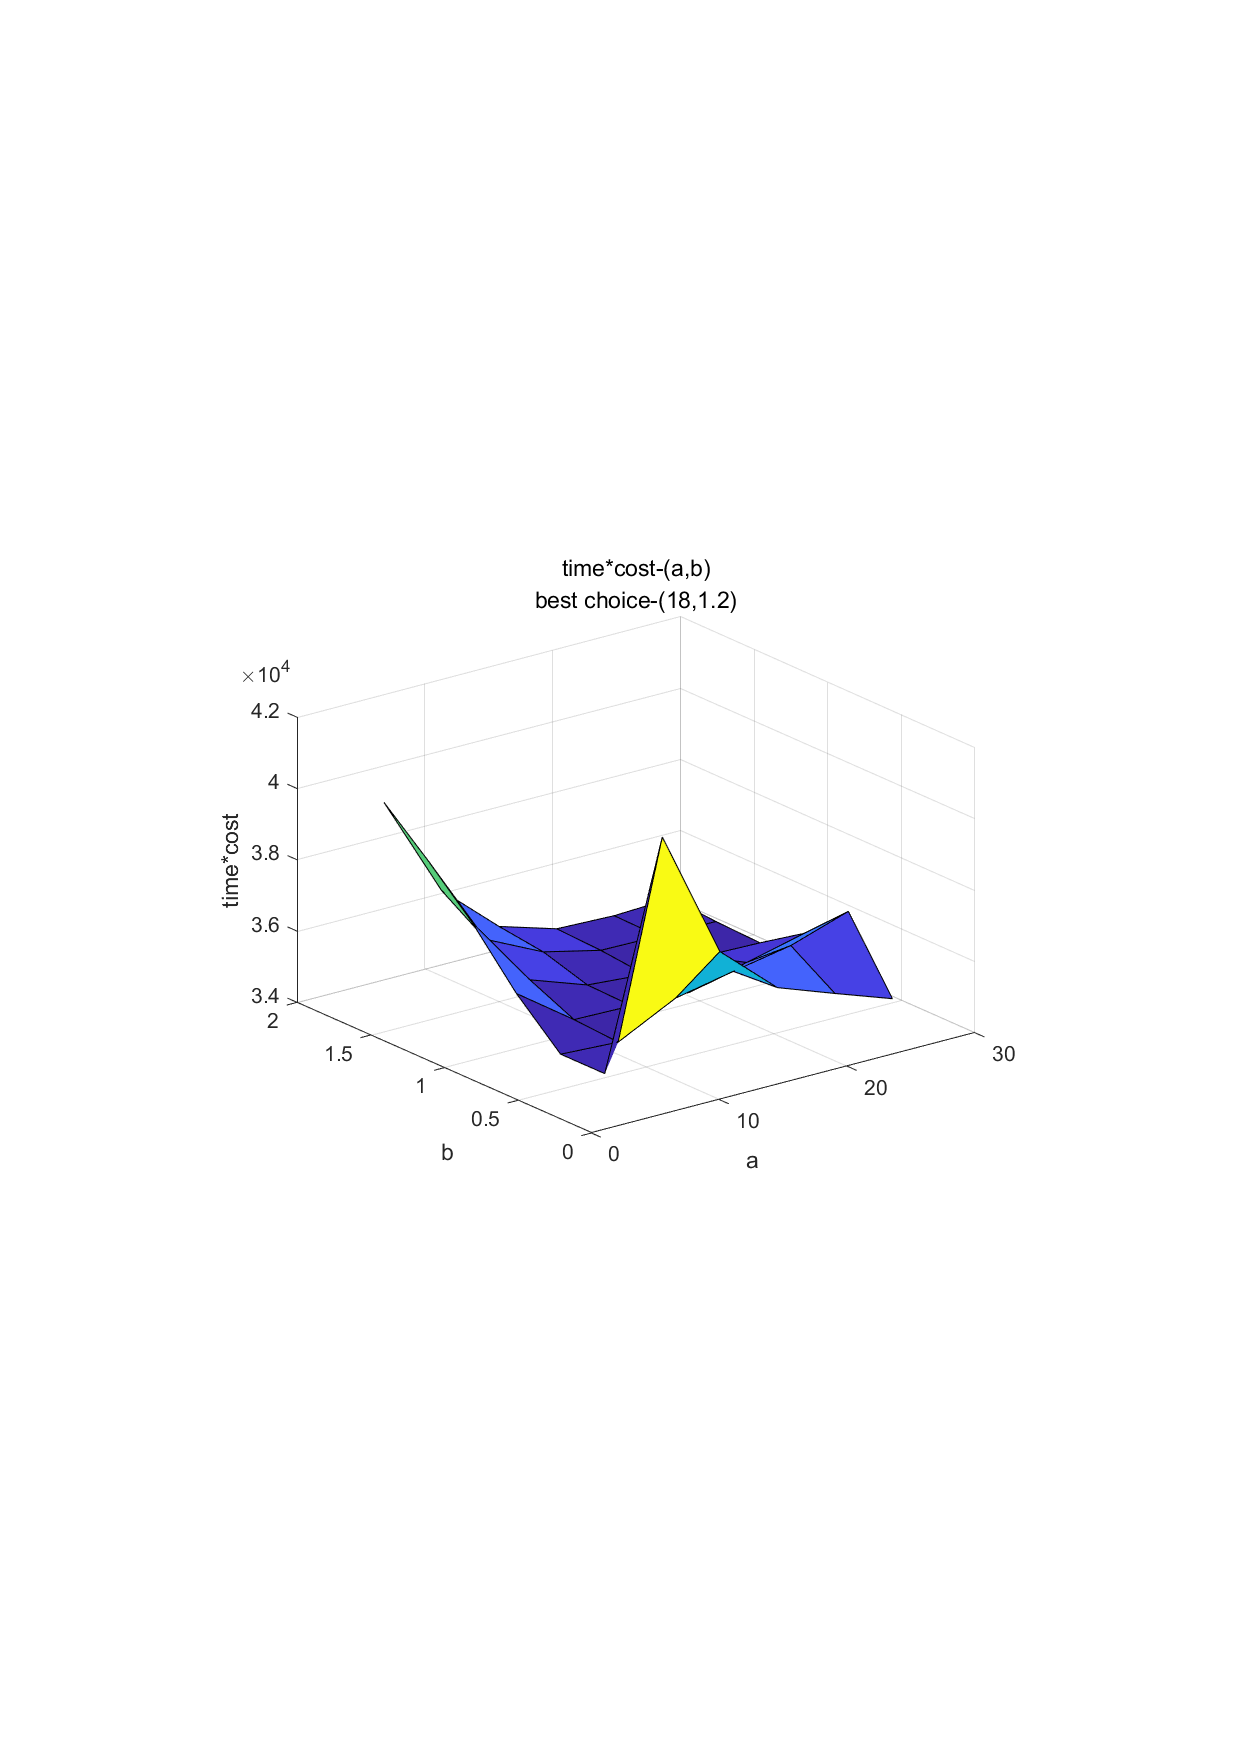
\includegraphics[width=\textwidth]{figure/ab}
		\caption{$time\times cost-(a,b)$}
		\label{fig:ab}
	\end{figure}

	In the figure weight of amount cost corresponds to $a$ and weight of time cost corresponds to $b$. Then we can see from the figure that the best choice of $a$ and $b$ is 4.5 and 1.8 respectively.

\subsection{Average Cost and Time}
We list the average cost and time achieved in each problem here in table \ref{tb:aveCT}. 
\begin{table}[H]
	\centering
	\begin{tabular}{|l|l|l|l|}
		\hline
		               &average cost     &  average time & number of hubs\\
		               \hline
		problem 1      &439.50                  &   1357.80& \\
		\hline
		problem 2      &437.94                  &   1369.31& 4 hubs\\
		\hline
		problem 3      &439.49                  &   1359.79& 32 hubs\\
		\hline
		problem 4      &969.08                  &   3374.58& \\
		\hline
	\end{tabular}
	\caption{Overall Evaluation}
	\label{tb:aveCT}
\end{table}

\indent From the table, we found some results:
\begin{enumerate}
	\item Problem 2 and 3 achieved lower $cost$ and $time$ than problem 1 because of the hubs. 
	\item In problem 3, much more hubs are constructed. This is because that this problem allows hub and substation exist in the same city.
	\item In problem 4, average cost and time are much larger than in problem 1. This is because not all cities are substations. Hence, longer delivery route is required.
\end{enumerate}

\section{Sensitivity Test}
In the program, we determine $c_0=3000$ and $c_1=300$. The 2 are parameters determining hub building cost. And we determine $x=0.7$. This is the ratio for hub transportation. And $capacity=1000$. This is the hub capacity.

In this section, we change the 4 parameters and observe their effect on our evaluation function $f=a\times cost+b\times time$.
\begin{enumerate}
	\item $c_0$ and $c_1$\par
	$\quad$ The achieved $f$ on different $c_0$ and $c_1$ is plotted in figure \ref{fig:c0} and \ref{fig:c1}. Select 2 neighbor points around the value using in the program. And we find that the slopes are 0 for both figure. This is because small change to these 2 parameters will not influence how we construct the hubs. Therefore, the model is not sensitive to these 2 parameters. But of course, we can see also in the figures that large change to these 2 parameters will still influence the result. 
	\begin{figure}
		\centering
		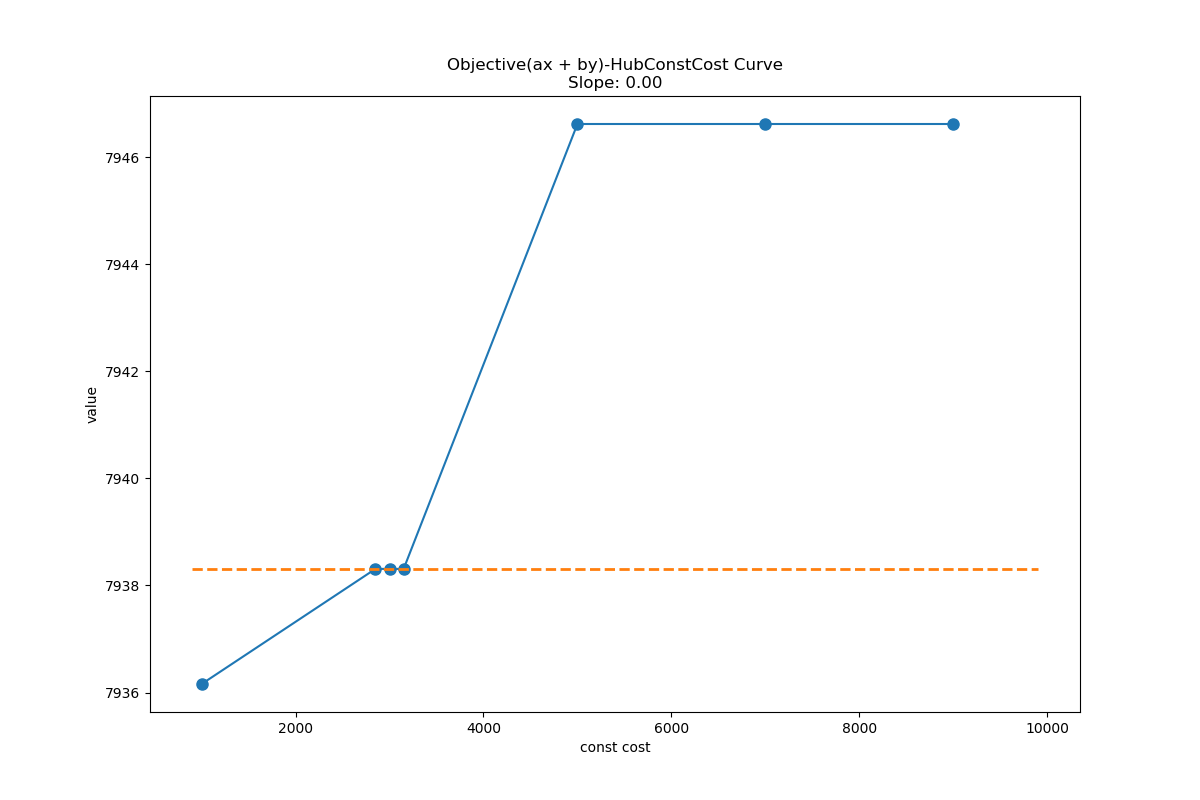
\includegraphics[width=\textwidth]{figure/const_cost.png}
		\caption{$f-c_0$}
		\label{fig:c0}
	\end{figure}
	\begin{figure}
		\centering
		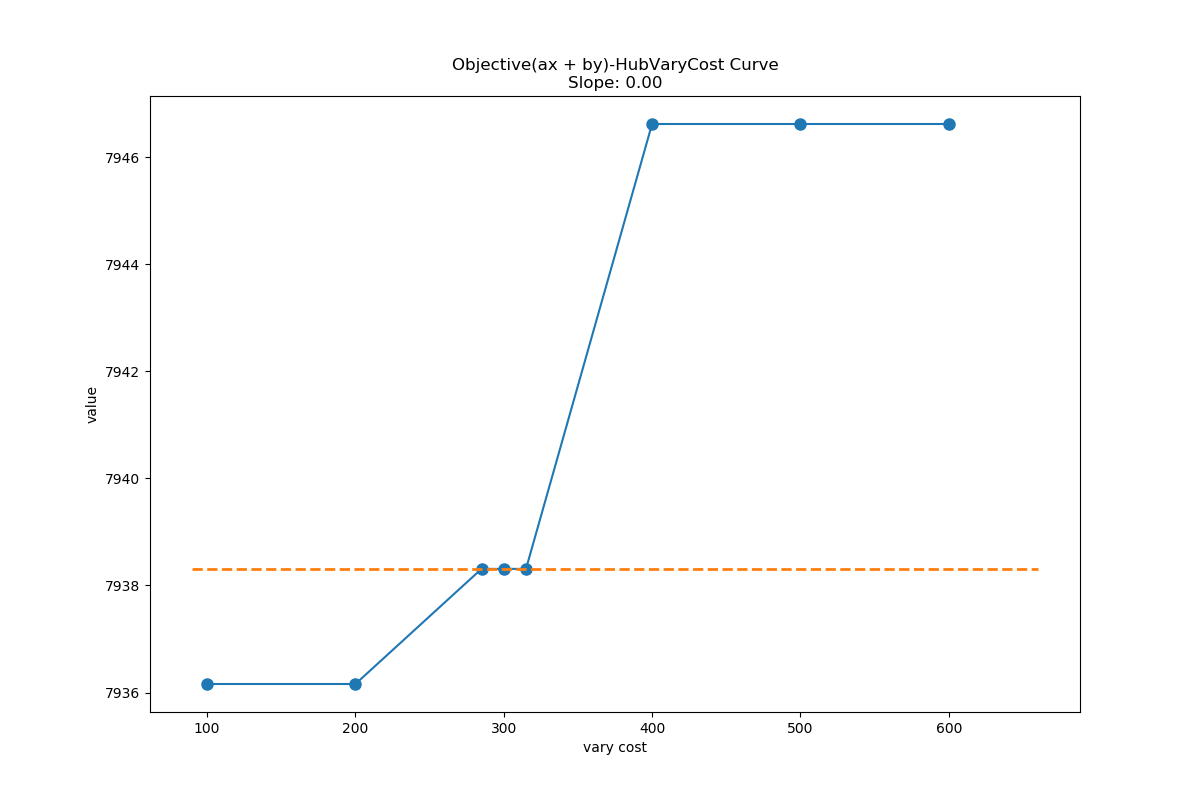
\includegraphics[width=\textwidth]{figure/vary_cost.png}
		\caption{$f-c_1$}
		\label{fig:c1}
	\end{figure}
	\item $x$
	The effect of $x$ is shown in figure \ref{fig:x}. We can see that the overall evaluation around $x=0.7$ is relatively stable. I.e. our model is also not sensitive to $x$ around our given value $0.7$. However, around lower value of $x$, our model is much more sensitive.
	\begin{figure}
		\centering
		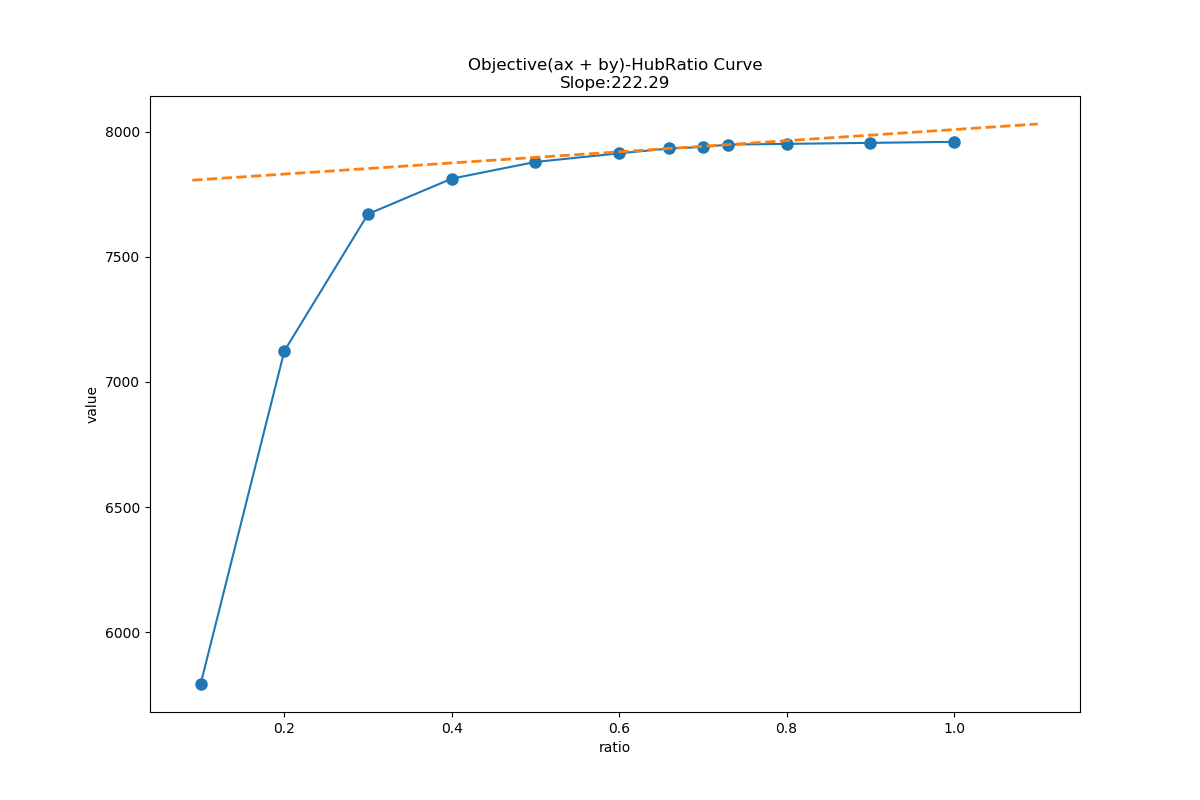
\includegraphics[width=\textwidth]{figure/x.png}
		\caption{$f-x$}
		\label{fig:x}
	\end{figure}
	\item $capacity$
	In problem 3, we give each hub restricted capacity.  Hence, we look into the effect of it also. The figure is given in figure \ref{fig:cap}. We can see that the slope is 0 around our given value 1000. This is also because small difference of parameters will not make changes to the hub construction. Hence, our model is not sensitive to $capacity$ as well.
	\begin{figure}
		\centering
		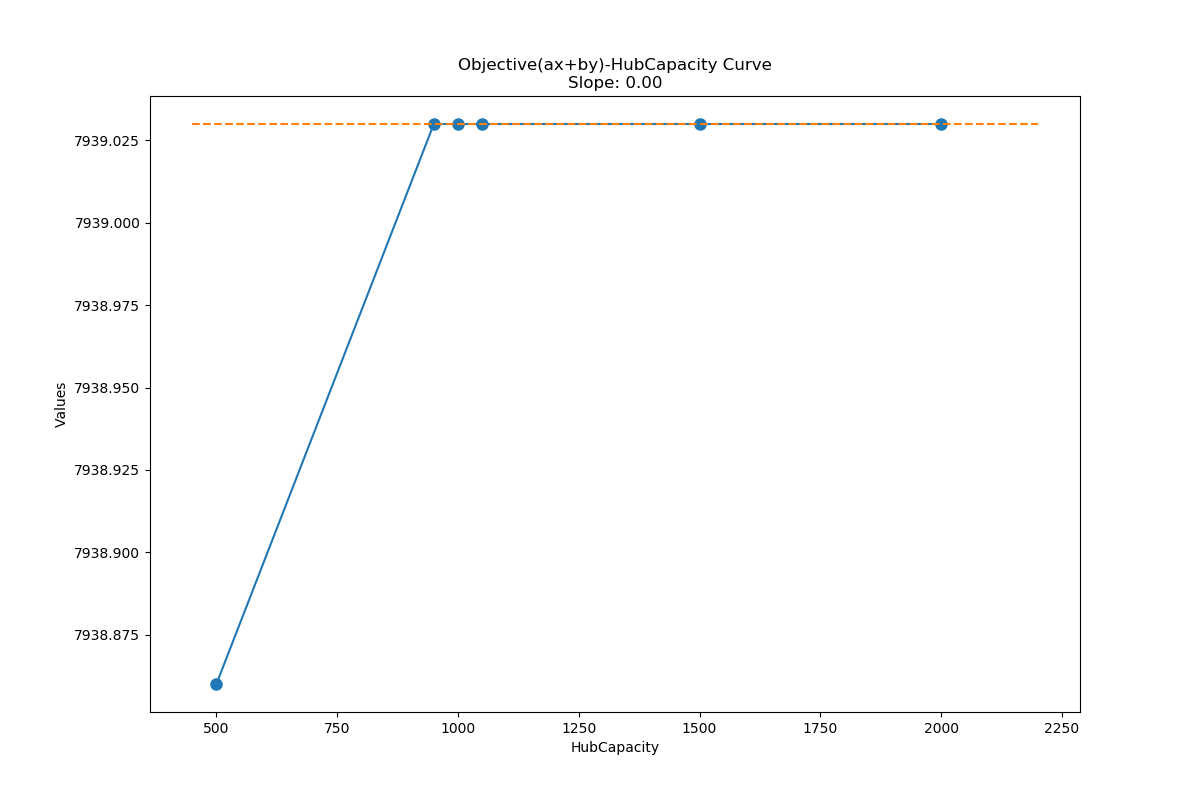
\includegraphics[width=\textwidth]{figure/capacity.png}
		\caption{$f-capacity$}
		\label{fig:cap}
	\end{figure}
\end{enumerate}

\section{Summary}
We refer to shortest path problem, sequential algorithm and knapsack problem to solve this project. And we sum the advantages and disadvantages of our model as follow:\\
\textbf{Disadvantages:} 
\begin{enumerate}
	\item In the worst case, the algorithms lead to poly-apx result in problem 2 and 3. And theoretically the algorithm can lead to arbitrarily bad result in problem 4. This may be far from the optimal. For problem 1, the ``approximation difference'' is also polynomial.
	\item Although the algorithm is poly-time algorithm, it's still not efficient enough. Especially for problem 2 and 3, it simulates the whole process in the worst case for a check. This needs very much time.
\end{enumerate}
\textbf{Advantages:}
\begin{enumerate}
	\item The algorithm works out very close solution to $OPT$ for problem 1 in practice. And it's efficient.
	\item In practice, the algorithms performs well. Because of the triangle inequility of real-world maps, the algorithm for problem 4 works out schemes very close to the optimal ones. For problem 2 and 3, the worst case seldom happens in practice. Hence the efficiency and performance are much better.
	\item All real-world objects (cities, transportation, $\cdots$) are all modeled to mathematical symbols. This helps the theoretical analysis and algorithm design.
\end{enumerate}

\newpage % Includes a new page
\pagenumbering{roman} 
\section{Acknowledgement}
From this project, we've learned very much. The largest achievement is that we've learned how to design algorithms in this project. And since we utilized the $dijskra$, sequential algorithm and $knapsack$ problem in this project, we become much more familiar to them. Also, as for the theoretical part, by proving the approximation ratio, we've got more familiar with the mathematical methods.

And from this project, we found that those problems in reality may seems simple. However, when we truly analyze them, investigate the algorithm, it turns out to be really hard. In problem 1, we find that the orders are independent with each other. And we thought we can solve the problem by processing the orders one by one. Then this becomes an easy problem. However, we struggled a lot to find such an algorithm and made many mistakes. And this problem even seems to be a NP complete one.

Thanks for professor Gao's instructions along the semester and the careful design of our labs and projects! We've really learned much from this course!


\newpage % Includes a new page
% Changes page numbering to roman page numbers
%\bibliography{literature}

%\bibliography{literature.bib} % Add the filename of your bibliography
%\bibliographystyle{apsr} % Defines your bibliography style

\begin{thebibliography}{99}
	\bibitem{1} Gao Xiaofeng. Slide12-ShortestPath. 2019
	
	\bibitem{2} Gao Xiaofeng. Slide15-NPReduction. 2019
	
	\bibitem{3} Gao Xiaofeng. Slide16-ApproximationI. 2019
	
	\bibitem{4} Gao Xiaofeng. Slide17-ApproximationII. 2019
\end{thebibliography}

\newpage % Includes a new page
\section*{Appendix} % Stars disable section numbers
% \appendix % Uncomment if you want to add an "automatic" appendix
Code is available on github. Website: https://github.com/dbgns/package-delivery\\
Model is available on website: http://resources.dbgns.com/package-delivery/models\\
The detailed result is available on website: http://resources.dbgns.com/package-delivery/results
\end{document}
